\documentclass{beamer}

\mode<presentation> {
\usetheme{Madrid}
}

\usepackage{graphicx} % Allows including images
\usepackage[utf8]{inputenc}
\usepackage[russian]{babel}
\usepackage{booktabs} % Allows the use of \toprule, \midrule and \bottomrule in tables

%----------------------------------------------------------------------------------------
%   TITLE PAGE
%----------------------------------------------------------------------------------------

\title[Acoustic fingerprinting]{Acoustic fingerprinting}

\author{Ayat Ospanov}
\institute[]
{
517th group \\
MMP, CMC, Lomonosov MSU \\
Moscow, Russia
}
\date{19.06.2017}

\begin{document}

\begin{frame}
\titlepage % Print the title page as the first slide
\end{frame}

%----------------------------------------------------------------------------------------
%   PRESENTATION SLIDES
%----------------------------------------------------------------------------------------

%------------------------------------------------
\section{First Section}
%------------------------------------------------

% \subsection{Subsection Example}

%------------------------------------------------

\begin{frame}
\frametitle{What is an acoustic fingerprint?}
\begin{itemize}
    \item Short summary of an audio object using a limited number of bits
\end{itemize}
\begin{center}
    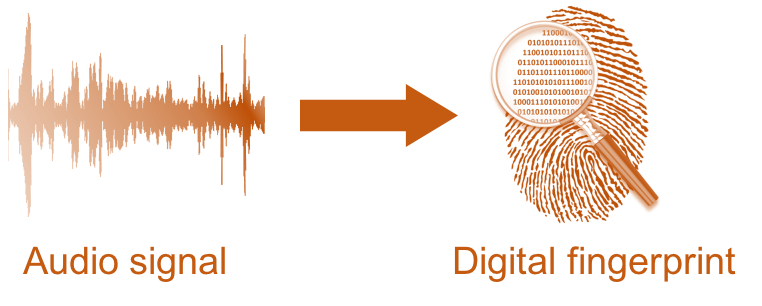
\includegraphics[width=0.8\linewidth]{pics/fingerprint}
\end{center}
\end{frame}

%------------------------------------------------

\begin{frame}
\frametitle{Why fingerprint?}
\begin{itemize}
    \item Efficient mechanism to establish the perceptual equality of two audio objects
    \item Advantages
    \begin{itemize}
        \item[-] Reduced memory/storage requirements
        \item[-] Efficient comparison
        \item[-] Efficient search
    \end{itemize}
\end{itemize}
\end{frame}

%------------------------------------------------

\begin{frame}
\frametitle{Example Systems}
\begin{itemize}
    \item Shazam
    \item SoundHound
    \item Google
    \item Chromaprint
    \item Echoprint
\end{itemize}
\end{frame}

%------------------------------------------------

\begin{frame}
\frametitle{Spectrograms}
\begin{itemize}
    \item Repeatedly use an Fast Fourier Transform (FFT) over small windows of time in samples to create a spectrogram
\end{itemize}
\begin{center}
    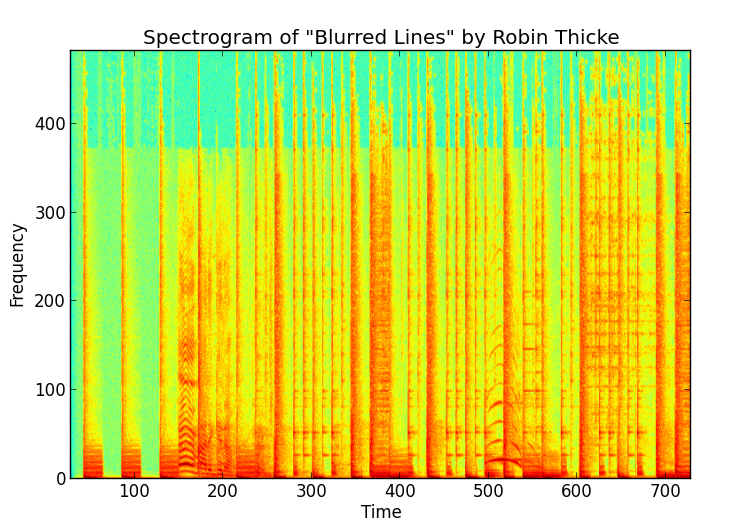
\includegraphics[width=0.75\linewidth]{pics/spectrogram}
\end{center}
\end{frame}

%------------------------------------------------

\begin{frame}
\frametitle{Peak Finding}
\begin{center}
    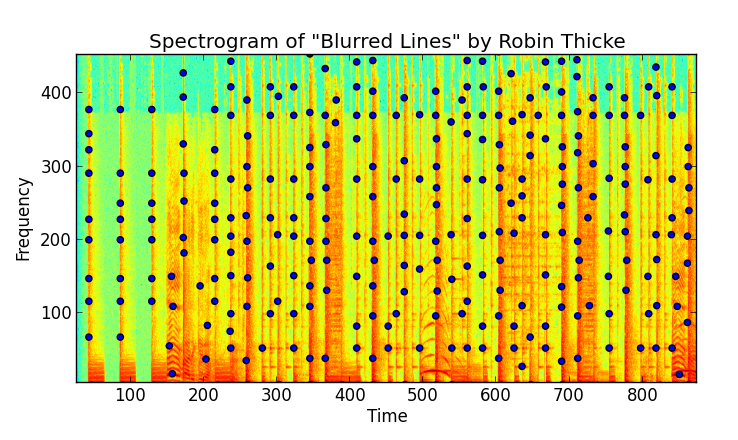
\includegraphics[width=\linewidth]{pics/spectrogram_peaks}
\end{center}
\end{frame}

%------------------------------------------------

\begin{frame}
\frametitle{Fingerprint hashing}
\begin{itemize}
    \item Audio fingerprinting is hashing of audio spectogram peaks
\end{itemize}

\begin{center}
    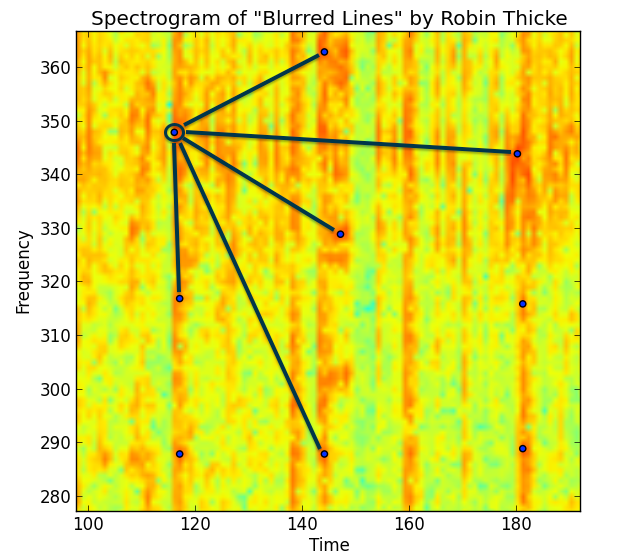
\includegraphics[width=0.6\linewidth]{pics/spectrogram_zoomed}
\end{center}
\end{frame}

%----------------------------------------------------------------------------------------

\end{document}
